\section{Auswertung}
\label{sec:Auswertung}

Die Messung der Apparaturkonstanten liefert 
\begin{align*}
  r_\text{K} = \SI{0.02683}{\metre}, \\ 
  m_\text{K} = \SI{0.14197}{\kilo\gram}, \\
  J_\text{K} = \frac{2}{5} m_\text{K} r_\text{K}^2 = 4,1 \cdot 10^{-5}\,\si{\kilo\gram\meter\squared}, \\
  N = 195, \\
  d = 0,138 \,\si{\meter}, \\
  R_\text{Spule} = 0,109 \,\si{\meter}.
\end{align*}

\subsection{Bestimmung des magnetischen Moments eines Magneten unter Ausnutzung der Gravitation}
Mithilfe von Gleichung (4) wird die Magnetfeldstärke ausgerechnet (Tabelle 1).
\begin{table}
\centering
\caption{Magnetfeldstärke $B$ in Abhängigkeit von Abstand $r$ und Spulenstrom $I$.}
\label{tab:bfeld}
\sisetup{table-format=1.2}
\begin{tabular}{c c c}
\toprule
\multicolumn{1}{c}{Abstand} & \multicolumn{1}{c}{Spulenstrom} & \multicolumn{1}{c}{Magnetfeldstärke} \\
{$r\:/\:\si{\centi\meter}$} & {$I\:/\:\si{\ampere}$} & $B\:/\:\si{\milli\tesla}$\\
\midrule
4,1 & 1,28 & 1,74 \\
4,9 & 1,49 & 2,02 \\
5,3 & 1,58 & 2,14 \\
5,6 & 1,6 & 2,17 \\
6,1 & 1,78 & 2,41 \\
7,2 & 2 & 2,71 \\
8,0 & 2,19 & 2,97 \\
8,9 & 2,35 & 3,19 \\
9,3 & 2,46 & 3,34 \\
10,1 & 2,64 & 3,58 \\
\bottomrule
\end{tabular}
\end{table}


\noindent Um das magnetische Moment der Kugel zu berechnen wird die Magnetfeldstärke $B$ gegen den Abstand 
$r$ aufgetragen und mithilfe linearer Regression in Form von 

\begin{align}
  y = a \cdot x + b, \\
  a = \frac{\overline{xy}-\overline{x}\cdot\overline{y}}{\overline{x^2}-\overline{x}^2}, \\
  b = \frac{\overline{x^2}\overline{y}-\overline{xy}\cdot\overline{x}}{\overline{x^2}-\overline{x}^2}
\end{align}
wird die Steigung der Ausgleichsgeraden bestimmt.

\begin{figure}
  \center
  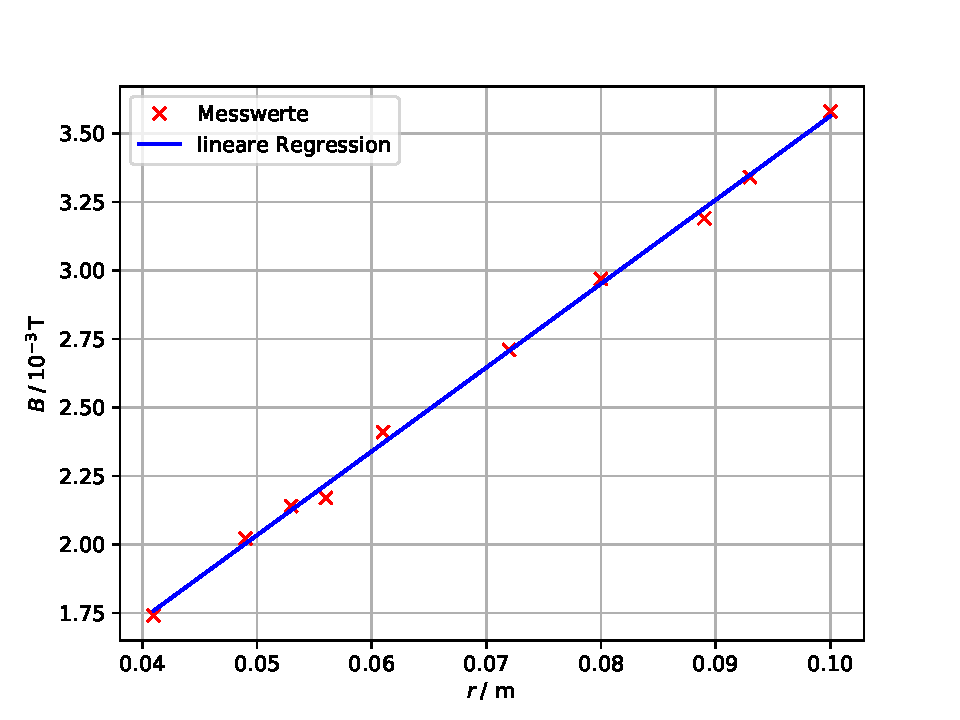
\includegraphics{feldstaerke.pdf}
  \caption{Magnetfeldstärke $B$ in Abhängigkeit des Abstands $r$.}
  \label{fig:feldstaerke}
\end{figure}

\noindent Nun wird nach Gleichung (7) das magnetische Moment $\mu_\text{Dipol}$ gemäß
\begin{gather}
\mu_\text{Dipol} = \frac{m_\text{g}g}{a}
\end{gather}
berechnet.
Mit
\begin{align*}
a = (0,0306 \pm 0,0005) \si{\kilo\gram\meter\per\second\squared\per\ampere\per\meter\squared}, \\
b = (0,0005 \pm 0,000034) \si{\kilo\gram\per\second\squared\per\ampere}
\end{align*}
folgt:
\begin{gather*}
\mu_\text{Dipol1} = (0,442 \pm 0,007)\,\si{\ampere\meter\squared}.
\end{gather*}

\subsection{Bestimmung des magnetischen Moments über die Schwingungsdauer eines Magneten}
Mittels Gleichung (4) wird erneut die Magnetfeldstärke $B$ der jeweiligen Stromstärke $I$ berechnet (Tabelle 2).
Um das magnetische Moment $\mu_\text{Dipol}$ zu berechnen wird $T^2$ gegen $1/B$ aufgetragen.
\begin{table}
\small
\centering
\caption{Zur Stromstärke $I$ zugehörige Magnetfeldstärke $B$, reziproke Magnetfeldstärke $\frac{1}{B}$, Periodendauer $T$ und quadrierte Periodendauer $T^2$.}
\label{tab:schwingung}
\begin{tabular}{c c c c c}
\toprule
\multicolumn{1}{c}{Spulenstrom} & \multicolumn{1}{c}{Magnetfeldstärke} & \multicolumn{1}{c}{reziproke Magnetfeldstärke} & \multicolumn{1}{c}{Periodendauer} & \multicolumn{1}{c}{quadrierte Periodendauer} \\
{$I\:/\:\si{\ampere}$} & {$B\:/\:\si{\milli\tesla}$} & {$\frac{1}{B}\:/\:\frac{1}{T}$} & {$T\:/\:\cdot 10^{-1}\si{\second}$} & {$T^2\:/\:\cdot 10^{-2}\si{\second\squared}$}\\
\midrule
3,8 & 5,15 & 194 & 8,46  & 71,57 \\
3,5 & 4,75 & 210 & 8,66  & 75,00 \\
3,2 & 4,34 & 230 & 8,86  & 78,50 \\
2,9 & 3,93 & 254 & 9,54  & 91,01 \\
2,6 & 3,53 & 283 & 10,05 & 101,00  \\
2,3 & 3,12 & 321 & 10,69 & 114,28  \\
2,0 & 2,71 & 369 & 11,45 & 131,10  \\
1,7 & 2,31 & 433 & 12,52 & 156,75  \\
1,4 & 1,90 & 526 & 13,76 & 189,34  \\
1,1 & 1,49 & 671 & 15,61 & 243,67  \\
\bottomrule
\end{tabular}
\end{table}

\begin{figure}[H]
  \center
  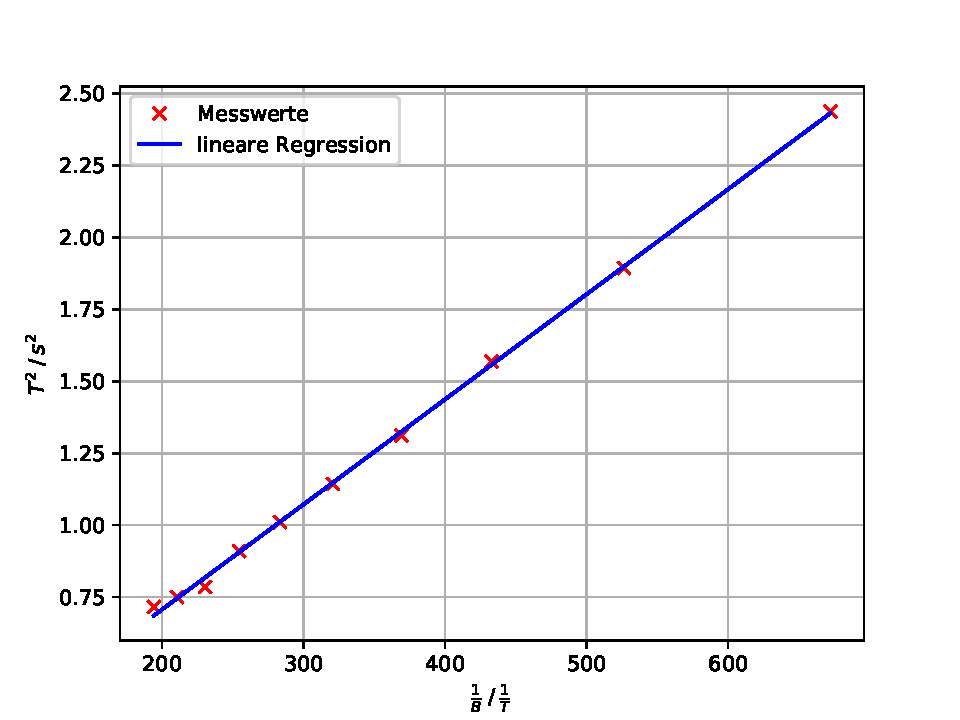
\includegraphics{schwingung.pdf}
  \caption{Quadrierte Schwingungsdauer $T^2$ in Abhängigkeit von der reziproken Magnetfeldstärke $1/B$}
  \label{fig:schwingung}
\end{figure}
\noindent Mittels linearer Regression (Abbildung 7) ergibt sich für die Ausgleichsgerade
\begin{align*}
a = (0,00365 \pm 0,00004)\,\si{\kilo\gram\per\ampere}, \\
b = (-0,023 \pm 0,014)\,\si{\second\squared}.
\end{align*}
Aus Gleichung (9) ergibt sich somit für das magnetische Moment
\begin{gather}
\mu_\text{Dipol2} = \frac{4\pi^2J_\text{K}}{a} = (0,443 \pm 0,005)\,\si{\ampere\meter\squared}.
\end{gather}

\subsection{Bestimmung des magnetischen Moments über die Präzession} %4.3
Um das magnetische Moment $\mu_\text{Dipol}$ zu bestimmen, wird die reziproke Periodendauer $1/T_\text{P}$
gegen die Magnetfeldstärke $B$ aufgetragen, welche sich aus der Stromstärke $I$ mittels Gleichung (4) ergibt.
\begin{table}
\centering
\caption{Zur Stromstärke $I$ zugehörige Magnetfeldstärke $B$ und reziproke Periodendauer $1/T_\text{P}$}
\label{tab:praezession}
\begin{tabular}{c c c}
\toprule
\multicolumn{1}{c}{Spulenstrom} & \multicolumn{1}{c}{Magnetfeldstärke} & \multicolumn{1}{c}{reziproke Periodendauer} \\
{$I\:/\:\si{\ampere}$} & {$B\:/\:\si{\milli\tesla}$} & {$1/T_\text{P}\:/\:\si{\per\second}$} \\
\midrule
0,2 & 0,27 & 0,0240 \\
0,5 & 0,68 & 0,0439 \\
0,8 & 1,08 & 0,0593 \\
1,1 & 1,49 & 0,0749 \\
1,4 & 1,90 & 0,0917 \\
1,7 & 2,31 & 0,1205 \\
2,0 & 2,71 & 0,1689 \\
2,3 & 3,12 & 0,1745 \\
2,6 & 3,53 & 0,2160 \\
2.8 & 3,80 & 0,2212 \\
\bottomrule
\end{tabular}
\end{table}
\begin{figure}
  \center
  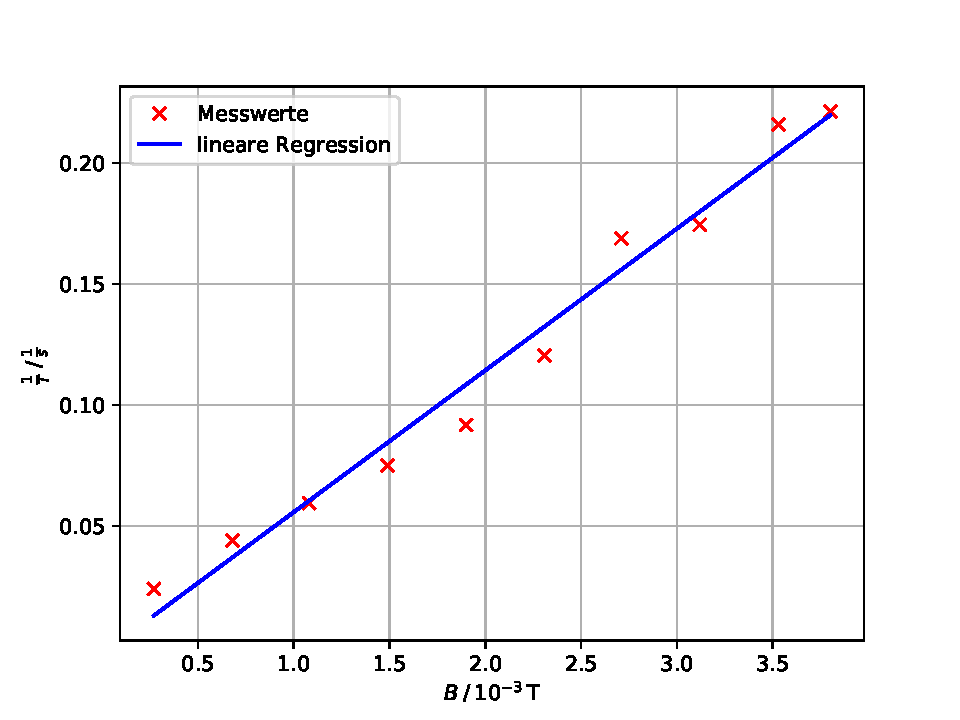
\includegraphics{praezession.pdf}
  \caption{Reziproke Periodendauer $1/T_\text{P}$ in Abhängigkeit von der Magnetfeldstärke $B$}
  \label{fig:praezession}
\end{figure}
\noindent Mithilfe der linearen Regression (Abbildung 8) ergibt sich für die Ausgleichsgerade
\begin{align*}
a = (58,6 \pm 3,1)\,\si{\ampere\second\per\kilo\gram}, \\
b = (-0,003 \pm 0,007)\,\frac{1}{s}.
\end{align*}
Aus der Steigung der Geraden lässt sich mittels
\begin{gather}
\mu_\text{Dipol} = 2\pi L_\text{K} a
\end{gather}
mit
\begin{gather*}
L_\text{K} = 4,1 \cdot 10^{-5} \si{\kilo\gram\meter\squared} \cdot 2\pi \cdot 4,3\si{\hertz} = 1,11 \cdot 10^{-3} \si{\kilo\gram\meter\squared\per\second}
\end{gather*}
das magnetische Moment
\begin{gather*}
\mu_\text{Dipol3} = (0,408 \pm 0,022)\,\si{\ampere\meter\squared}.
\end{gather*}
berechnen.